% Shorter slides for EES403 Group 1, based on the IISER Mohali Beamer template.
% Do not edit slides_shorter.tex or slides_shorter_notes.tex: scripts/build_latex.py generates
% them from this file and fills every double-angle placeholder from results/tables.
%
% Nine content slides for a talk of about 10 minutes (timed at about 145 words per minute). Title, section dividers, the closing
% "Questions" frame and the references are transitions and are not counted.
% Speakers: Sangeeta (Introduction; Conclusions), Sangam (Data), Pranay (Methods, all of the
% mathematics), Aparna (Results I), Robin (Results II). Only Pranay's notes use equations.
% Every note starts with [speaker | time on this slide | clock at the end of the slide].
\documentclass[aspectratio=169, 11pt]{beamer}
\usetheme{Boadilla}
\usecolortheme{seahorse}
\usefonttheme{serif}

\usepackage{graphicx,xcolor}
\usepackage{amsmath,amssymb,amsfonts}
\usepackage{booktabs}
\usepackage{adjustbox}  % trim figures by a fraction of their size
\usepackage{pgfpages}
\usepackage[round]{natbib}
\pdfinfoomitdate=1   % no creation date in the PDF metadata
\pdftrailerid{}
%NOTES-OPTION%

\setbeamertemplate{navigation symbols}{}
\setbeamerfont{note page}{size=\small}
\setbeamertemplate{note page}[plain]
\setbeamertemplate{section in toc}[sections numbered]
\graphicspath{{images/}{../../results/figures/}{../../results/figures/slides/}{../../docs/}}

\definecolor{lpcol}{HTML}{1F5A96}
\definecolor{hpcol}{HTML}{A3236B}

\newcommand{\takeaway}[1]{\vfill\begin{block}{}\centering #1\end{block}}
\newcommand{\source}[1]{\par\vspace{1pt}{\tiny\color{gray}#1}}
\newcommand{\presenter}{}
\newcommand{\speaker}[1]{\renewcommand{\presenter}{#1}}

% Section divider (a transition, not a content slide): section name and presenter.
\AtBeginSection[]{
  \begin{frame}[plain, noframenumbering]
  \vfill
  \begin{center}
  {\usebeamercolor[fg]{structure}\Large\bfseries \insertsectionhead}\\[6pt]
  {\normalsize Presented by \textbf{\presenter}}
  \end{center}
  \vfill
  \end{frame}
}

\title[LPF vs HPF on Sentinel-2]{Low-pass and High-pass Filtering\\of Sentinel-2 Imagery over the Aravalli Ridge}
\subtitle{Which filtering technique suits which remote sensing application?}
\author[Group 1, EES403]{\textbf{Group 1}\\[2pt]
  {\footnotesize Pranay Chakraborty (MS22041),\ Sangeeta Kumari (PH25084),\ Aparna Manoj (MS24070),\\
   Robin (MS23138),\ Sangam (MS23222)}}
\institute[IISER Mohali]{\footnotesize EES403: Advanced Remote Sensing and GIS\\
  Instructors: Dr.\ Chandrakant Ojha and Dr.\ Meenakshi Devi\\[2pt]
  Indian Institute of Science Education and Research, Mohali}
\date{}
\titlegraphic{\vspace{-9mm}
\includegraphics[width=1.3cm]{iiserm_logo.jpg}}

\begin{document}

\begin{frame}[plain]
\titlepage
\end{frame}
\note{[Sangeeta | 0:15 | 0:15]\\
Good morning. We are Group 1. We compared low-pass and high-pass filtering on a Sentinel-2 image of the Aravalli ridge, to find out which kind of filter suits which remote sensing job.}

% ================================================================== Introduction (Sangeeta)
\speaker{Sangeeta}
\section{Introduction}

% ------------------------------------------------------------------ content slide 1
\begin{frame}{Low-pass smooths, high-pass sharpens: which one, for what?}
\begin{columns}[T]
\column{0.36\textwidth}
\small
\textbf{Spatial frequency}: how often brightness changes per unit distance \citep{lillesand2015}.

\medskip
\textcolor{lpcol}{\textbf{Low-pass}} keeps slow change\\ {\footnotesize fields, water $\Rightarrow$ smoother image, less noise}

\medskip
\textcolor{hpcol}{\textbf{High-pass}} keeps fast change\\ {\footnotesize roads, ridge crests $\Rightarrow$ edges stand out}

\medskip
\footnotesize We test both on five jobs: noise removal, land-cover classification, edges and lineaments, change to the spectra, speed.
\column{0.62\textwidth}
\adjincludegraphics[trim={{0.27\width} 0 0 0}, clip, width=\textwidth]{fig06_line_profile.png}
\source{NIR reflectance along a 1.6 km line on the ridge: original (black), low-pass (blue), high-boost (pink).}
\end{columns}
\end{frame}
\note{[Sangeeta | 0:45 | 1:00]\\
A satellite image is a grid of brightness values. Over a field or a lake the values change slowly; across a road or a ridge crest they jump within a few pixels. A low-pass filter keeps the slow changes and gives a smoother image. A high-pass filter keeps the fast changes, so edges stand out. The plot is real data along one line on the ridge: the black line is the original, the blue lines are flatter after smoothing, and the pink lines are steeper after sharpening. The two filters do opposite jobs, so we did not look for one winner. We tested them on five jobs and picked the best filter for each.}

% ================================================================== Data (Sangam)
\speaker{Sangam}
\section{Study Area and Data}

% ------------------------------------------------------------------ content slide 2
\begin{frame}{One winter scene holds ridges, city and farmland}
\centering
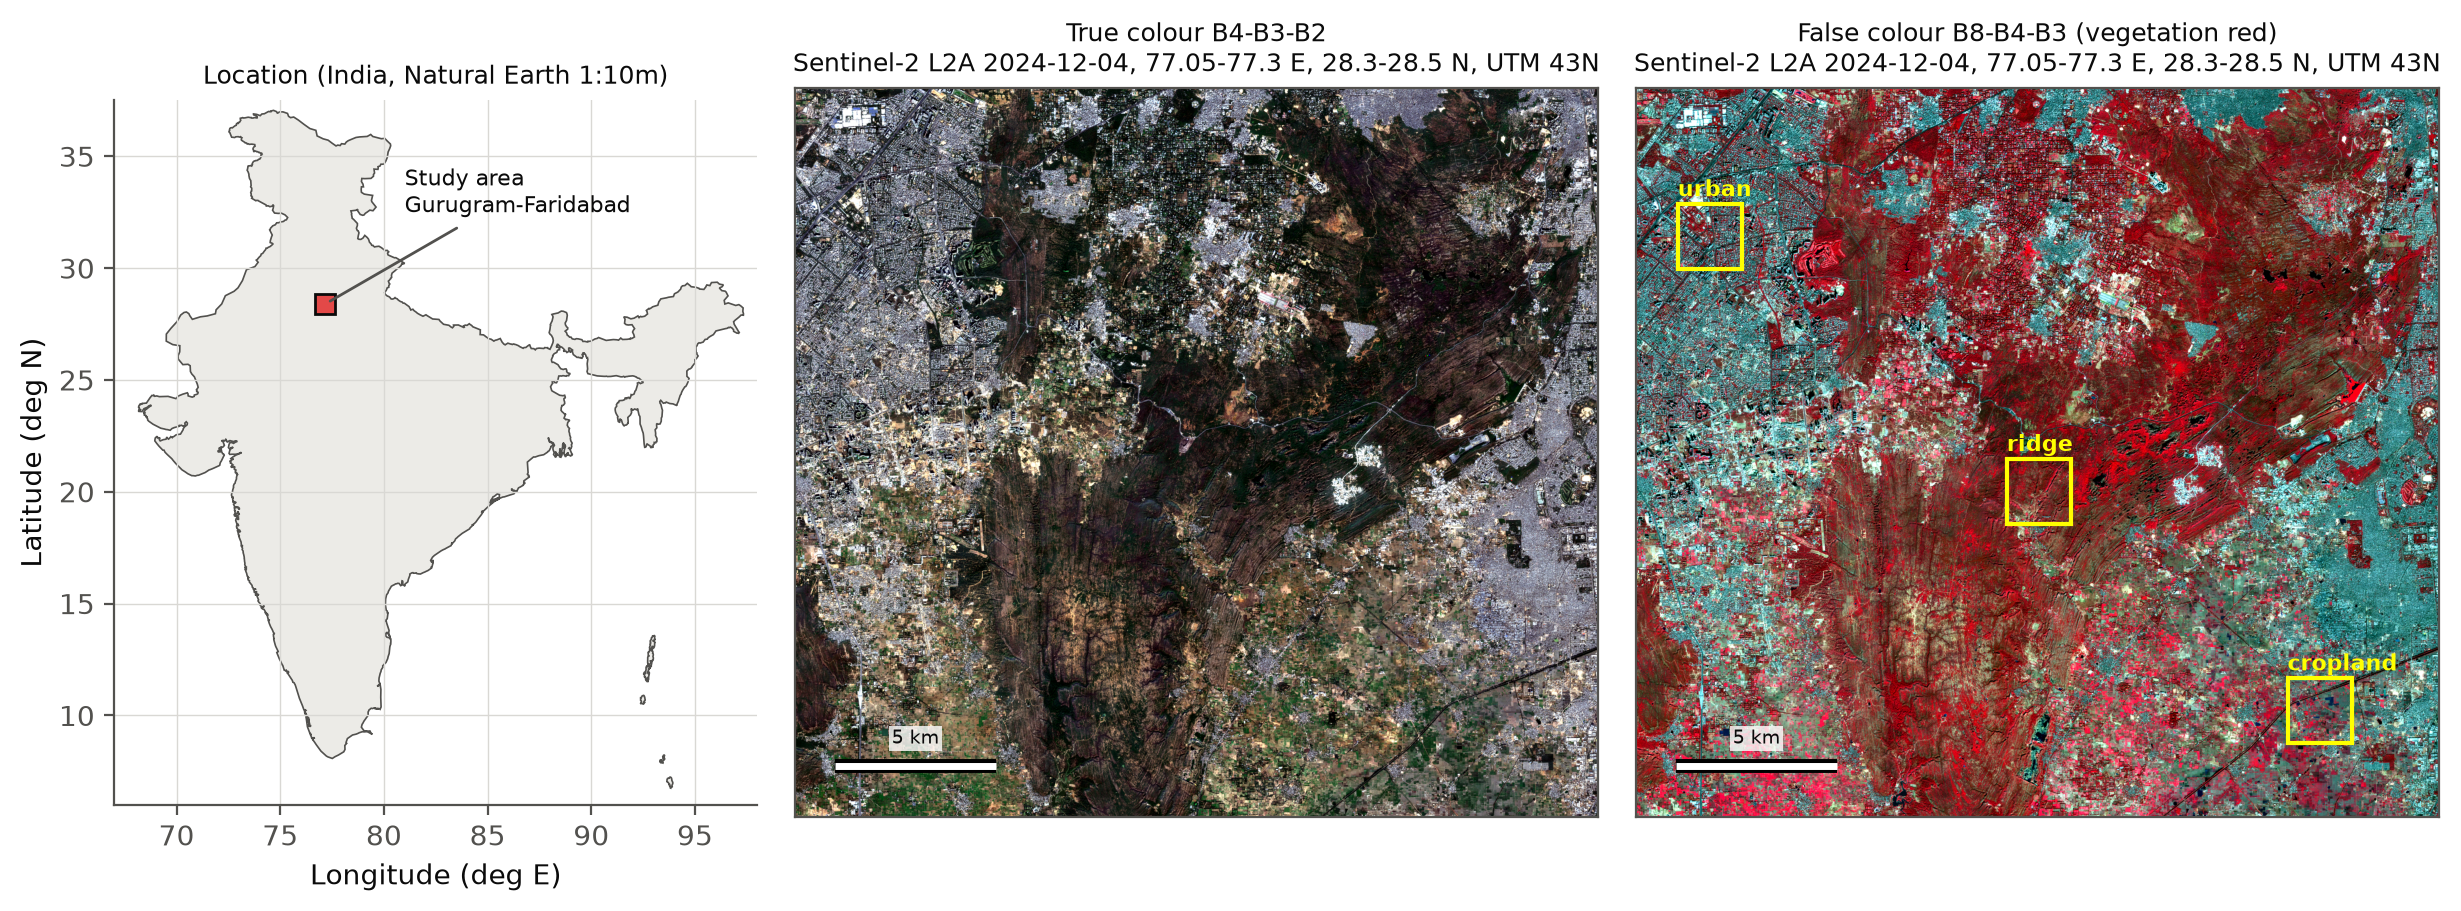
\includegraphics[width=0.78\textwidth]{fig01_study_area.png}
\source{Left: location. Centre: true colour. Right: false colour, vegetation red. Yellow boxes: ridge, urban and cropland windows.}

\vspace{4pt}
\scriptsize
\begin{tabular}{@{}ll@{\hspace{6mm}}ll@{}}
\toprule
Image & Sentinel-2 L2A, <<acq_date>>, tile <<tile>> & Area & 25 $\times$ 23 km, <<width>> $\times$ <<height>> px \\
Bands & blue, green, red, near-infrared (10 m) & Cloud and haze & <<bad_pct>>\% (best of <<n_candidates>> scenes) \\
Reference map & ESA WorldCover 2021, 5 classes & Water & <<water_pct>>\% of area, dropped \\
\bottomrule
\end{tabular}
\end{frame}
\note{[Sangam | 1:00 | 2:00]\\
Our area is a 25 by 23 kilometre box between Gurugram and Faridabad. We chose it because one image holds very different textures: the rocky Aravalli ridges with long straight features, the dense streets of Gurugram, and smooth crop fields in the south-east. The yellow boxes are the three small windows we zoom into later. The image is Sentinel-2, taken on <<acq_date>>, using the blue, green, red and near-infrared bands at 10 metre pixels. We looked at <<n_candidates>> winter scenes and picked the one with the least cloud and haze inside our box, only <<bad_pct>> percent. To check classification and boundaries we used the ESA WorldCover land-cover map. Water covered only <<water_pct>> percent of the area, so it was dropped, leaving five classes. WorldCover is itself made by a computer model, so we treat it as a reference, not as the truth. Pranay will explain how the filters work.}

% ================================================================== Methods (Pranay)
\speaker{Pranay}
\section{Methods}

% ------------------------------------------------------------------ content slide 3
\begin{frame}{Spatial domain: each output pixel is a weighted sum of its neighbours}
\begin{equation*}
g(x,y) \;=\; \sum_{s=-a}^{a}\;\sum_{t=-b}^{b} w(s,t)\; f(x-s,\; y-t)
\end{equation*}
\vspace{-4pt}\centering{\footnotesize computed by shift and accumulate over the kernel cells, with mirror padding at the border}\par
\footnotesize
\begin{columns}[T]
\column{0.47\textwidth}
\begin{block}{Low-pass}
Mean $n\times n$: $w = 1/n^2$,\; $n = 3,5,7,9$\\[2pt]
Gaussian: $w(s,t)\propto \exp\!\big(-\tfrac{s^2+t^2}{2\sigma^2}\big)$, $\sum w = 1$, $\sigma=1,2,3$\\[2pt]
Median $3\times3$, $5\times5$: non-linear, ignores single spikes
\end{block}
\column{0.51\textwidth}
\begin{block}{High-pass}
$\text{HPF}_n = f - \text{mean}_{n\times n}(f)$ \hfill \citep{lillesand2015}\\[2pt]
Laplacian $\begin{bmatrix}0&1&0\\1&-4&1\\0&1&0\end{bmatrix}$;\; Sobel, Prewitt: $\sqrt{G_x^2+G_y^2}$\\[2pt]
High-boost: $f + k\cdot\text{HPF}_n$,\; $k = 0.5, 1, 1.5$
\end{block}
\end{columns}
\source{Written in NumPy; unit tests against \texttt{scipy.ndimage} agree to $<10^{-5}$. \citet{gonzalez2018}, Ch.\ 3.}
\end{frame}
\note{[Pranay | 1:25 | 3:25]\\
In the spatial domain each output pixel g is a weighted sum of the input pixels f around it, with the weights in a kernel w. Strictly this is a convolution, which rotates the kernel by 180 degrees, but our kernels are symmetric so it makes no difference. Our code loops over the kernel cells rather than the pixels: for each cell it shifts the whole mirror-padded image, multiplies by the weight and adds it to the output, so the cost grows with n squared. On the low-pass side, the mean gives equal weights of one over n squared; the Gaussian gives nearer pixels more weight, with the weights summing to one so brightness is kept; the median takes the middle value of the window, so a single spike is ignored. On the high-pass side, the classic remote sensing HPF is the image minus its mean filter. The Laplacian is a second derivative, and Sobel and Prewitt estimate the first derivatives G x and G y, from which we take the gradient magnitude. High-boost adds k times the HPF back to the image. We wrote all of these in NumPy and checked them against SciPy; the largest difference is below ten to the minus five.}

% ------------------------------------------------------------------ content slide 4
\begin{frame}{Frequency domain: filtering is a multiplication of the spectrum}
\begin{columns}[T]
\column{0.54\textwidth}
\small
\[ g = \mathcal{F}^{-1}\big\{ H(u,v)\cdot\mathcal{F}\{f\}\big\} \]
\footnotesize
$D$: distance from spectrum centre, $D=1$ at Nyquist; $D_0 = 0.1, 0.2, 0.3$
\[
\begin{array}{ll}
\text{Ideal:} & H = 1 \text{ if } D\le D_0, \text{ else } 0\\[2pt]
\text{Butterworth } (n=2): & H = 1/\big(1+(D/D_0)^{4}\big)\\[2pt]
\text{Gaussian:} & H = \exp\!\big(-D^2/2D_0^2\big)\\[2pt]
\text{High-pass:} & H_{\text{HP}} = 1 - H
\end{array}
\]
Gaussian mask $\equiv$ spatial Gaussian with $\sigma = 1/(\pi D_0)$ px\\[3pt]
Ideal mask: sharp cut $\Rightarrow$ sinc kernel $\Rightarrow$ ringing ($\approx 9\%$ overshoot)
\column{0.44\textwidth}
\adjincludegraphics[trim={0 0 0 {0.50\height}}, clip, width=\textwidth]{fig03_fft_spectra.png}
\source{Log-magnitude spectra of the NIR crop: original, Gaussian LPF, Gaussian HPF ($D_0=0.1$).}

\smallskip
\footnotesize In total <<n_filters>> filter settings, plus the course example (square ideal masks of 61, 91, 121 px).
\end{columns}
\end{frame}
\note{[Pranay | 1:10 | 4:35]\\
By the convolution theorem, convolution in space is multiplication in frequency. So we take the Fourier transform, multiply by a mask H, and transform back. We mirror-pad first, because the FFT treats the image as periodic and the left edge would otherwise leak into the right. D is the distance from the centre of the spectrum, scaled to one at the Nyquist frequency, and D0 is the cutoff. The ideal mask is a hard cut, Butterworth rolls off smoothly, Gaussian more smoothly still, and each high-pass mask is one minus its low-pass mask. On the right, the low-pass keeps the bright centre and the high-pass removes it. Two results from theory: a Gaussian mask with cutoff D0 is the same filter as a spatial Gaussian with sigma one over pi D0, which links the two domains; and a hard cut in frequency is a sinc kernel in space, whose negative side lobes cause ripples beside edges, about nine percent overshoot. Aparna will show both on our data. Altogether we ran <<n_filters>> filter settings.}

% ------------------------------------------------------------------ content slide 5
\begin{frame}{How each experiment is scored}
\footnotesize
\begin{tabular}{@{}lp{3.9cm}p{8.4cm}@{}}
\toprule
 & Question & Deciding measure \\
\midrule
E1 & Noise removal & $\text{PSNR} = 10\log_{10}(1/\text{MSE})$ dB on a noisy crop; also SSIM \citep{wang2004} \\
E2 & Land-cover classification & Random Forest \citep{breiman2001}; Cohen's $\kappa = (p_o - p_e)/(1-p_e)$; salt-and-pepper index \\
E3 & Edges and lineaments & Canny \citep{canny1986} edge F1 vs WorldCover boundaries; ridge coherence $C = \dfrac{\lambda_1-\lambda_2}{\lambda_1+\lambda_2}$ \\
E4 & Change to the spectra & spectral angle $\text{SAM} = \arccos\dfrac{\mathbf{x}\cdot\mathbf{y}}{|\mathbf{x}||\mathbf{y}|}$; $|\Delta\text{NDVI}|$ \\
E5 & Speed & median of 5 runs on one full band, spatial vs FFT \\
\bottomrule
\end{tabular}
\takeaway{\small E2 uses a \textbf{spatially blocked split} (128 px blocks, 70/30) so test pixels are not near-copies of training pixels.}
\end{frame}
\note{[Pranay | 1:10 | 5:45]\\
Each experiment has one deciding measure. PSNR is ten log ten of one over the mean squared error, since reflectance runs from zero to one; three decibels more is about half the error. Cohen's kappa is the observed agreement p o corrected for the agreement p e expected by chance. For edges we use the F1 score of Canny edges against WorldCover boundaries, and for the ridge we use coherence from the structure tensor: lambda one and lambda two are its eigenvalues, so C is near one when the gradients share one direction, as along parallel ridges, and near zero for speckle. The spectral angle is the angle between a pixel's four-band vector before and after filtering; zero means the shape of the spectrum is unchanged. For classification we split the area into 128 pixel blocks and divide the blocks 70 to 30, because neighbouring pixels are almost identical and a random pixel split would inflate the accuracy. Aparna will now show the results.}

% ================================================================== Results I (Aparna)
\speaker{Aparna}
\section{Results I: What the Filters Do}

% ------------------------------------------------------------------ content slide 6
\begin{frame}{Low-pass blurs the street grid; high-boost makes it crisper}
\centering
% panel titles strip + Gurugram row of each figure (the ridge row is in the full deck)
\adjincludegraphics[trim={0 {0.954\height} 0 0}, clip, width=0.96\textwidth]{slide_lpf.png}\\[-1pt]
\adjincludegraphics[trim={0 0 0 {0.515\height}}, clip, width=0.96\textwidth]{slide_lpf.png}\\[4pt]
\adjincludegraphics[trim={0 {0.955\height} 0 0}, clip, width=0.66\textwidth]{slide_highboost.png}\\[-1pt]
\adjincludegraphics[trim={0 0 0 {0.52\height}}, clip, width=0.66\textwidth]{slide_highboost.png}
\source{Gurugram window, false colour, same stretch. Top: low-pass filters. Bottom: high-boost (original plus a share of the edge layer).}
\end{frame}
\note{[Aparna | 0:50 | 6:35]\\
This is a two kilometre window over Gurugram, with the same colours in every panel. The top row shows the smoothing filters. All of them blur the streets and building edges. The median keeps straight edges a little sharper, because it picks a real value instead of averaging across the edge. The Gaussian done in the frequency domain, on the far right, looks just like the ordinary Gaussian, as Pranay said it should. The bottom row shows high-boost, which adds the edge layer back onto the image. As the strength goes up, boundaries get crisper and the colours stay the same. At the strongest setting, on the right, bright and dark outlines start to appear around buildings, so a moderate strength is better.}

% ------------------------------------------------------------------ content slide 7
\begin{frame}{The ideal mask rings; the median is best for impulse noise}
\begin{columns}[T]
\column{0.55\textwidth}
\adjincludegraphics[trim={{0.25\width} 0 0 {0.52\height}}, clip, width=\textwidth]{fig05_ringing.png}
\source{Clean step edge passed through each mask, $D_0 = 0.1$.}

\footnotesize
\begin{tabular}{@{}lccc@{}}
\toprule
Mask & Ideal & Butterworth & Gaussian \\
\midrule
Overshoot (\% of step) & \textbf{<<ring_ideal>>} & <<ring_butter>> & <<ring_gauss>> \\
\bottomrule
\end{tabular}
\column{0.43\textwidth}
\begin{block}{E1: noise removal (PSNR, higher is better)}
\footnotesize
\textbf{Salt-and-pepper noise}\\
noisy <<e1_sp_noisy>> dB $\rightarrow$ median $3\times3$ \textbf{<<e1_sp_best_psnr>> dB}\\
best averaging filter: <<e1_sp_lin_psnr>> dB

\medskip
\textbf{Random noise}\\
noisy <<e1_g_noisy>> dB $\rightarrow$ <<p:e1_g_best>> \textbf{<<e1_g_best_psnr>> dB}\\
<<e1_g_n_worse>> of <<e1_g_n_lpf>> low-pass filters made it worse
\end{block}
\end{columns}
\takeaway{\small Use smooth masks, not the ideal one. Use the median for spikes, and only light smoothing for random noise.}
\end{frame}
\note{[Aparna | 1:00 | 7:35]\\
On the left we passed a clean step, a jump from dark to bright, through the three frequency masks. The ideal mask produces ripples on both sides and overshoots by <<ring_ideal>> percent of the step, which matches what Pranay predicted. Butterworth overshoots by <<ring_butter>> percent and Gaussian by <<ring_gauss>>. So the ideal mask should be avoided. On the right is the noise test, where higher PSNR means closer to the clean image. With salt-and-pepper noise, which is scattered single bad pixels, the 3 by 3 median raised the score from <<e1_sp_noisy>> to <<e1_sp_best_psnr>>, far ahead of any averaging filter, because averaging spreads each bad pixel over its neighbours while the median simply throws it away. With random noise, only the lightest filters helped; <<e1_g_n_worse>> of the <<e1_g_n_lpf>> smoothing filters made the image worse, because they removed more real detail than noise. Robin will present the other experiments.}

% ================================================================== Results II (Robin)
\speaker{Robin}
\section{Results II: Classification, Edges and Cost}

% ------------------------------------------------------------------ content slide 8
\begin{frame}{Smoothing helps classification; sharpening helps edges}
\centering
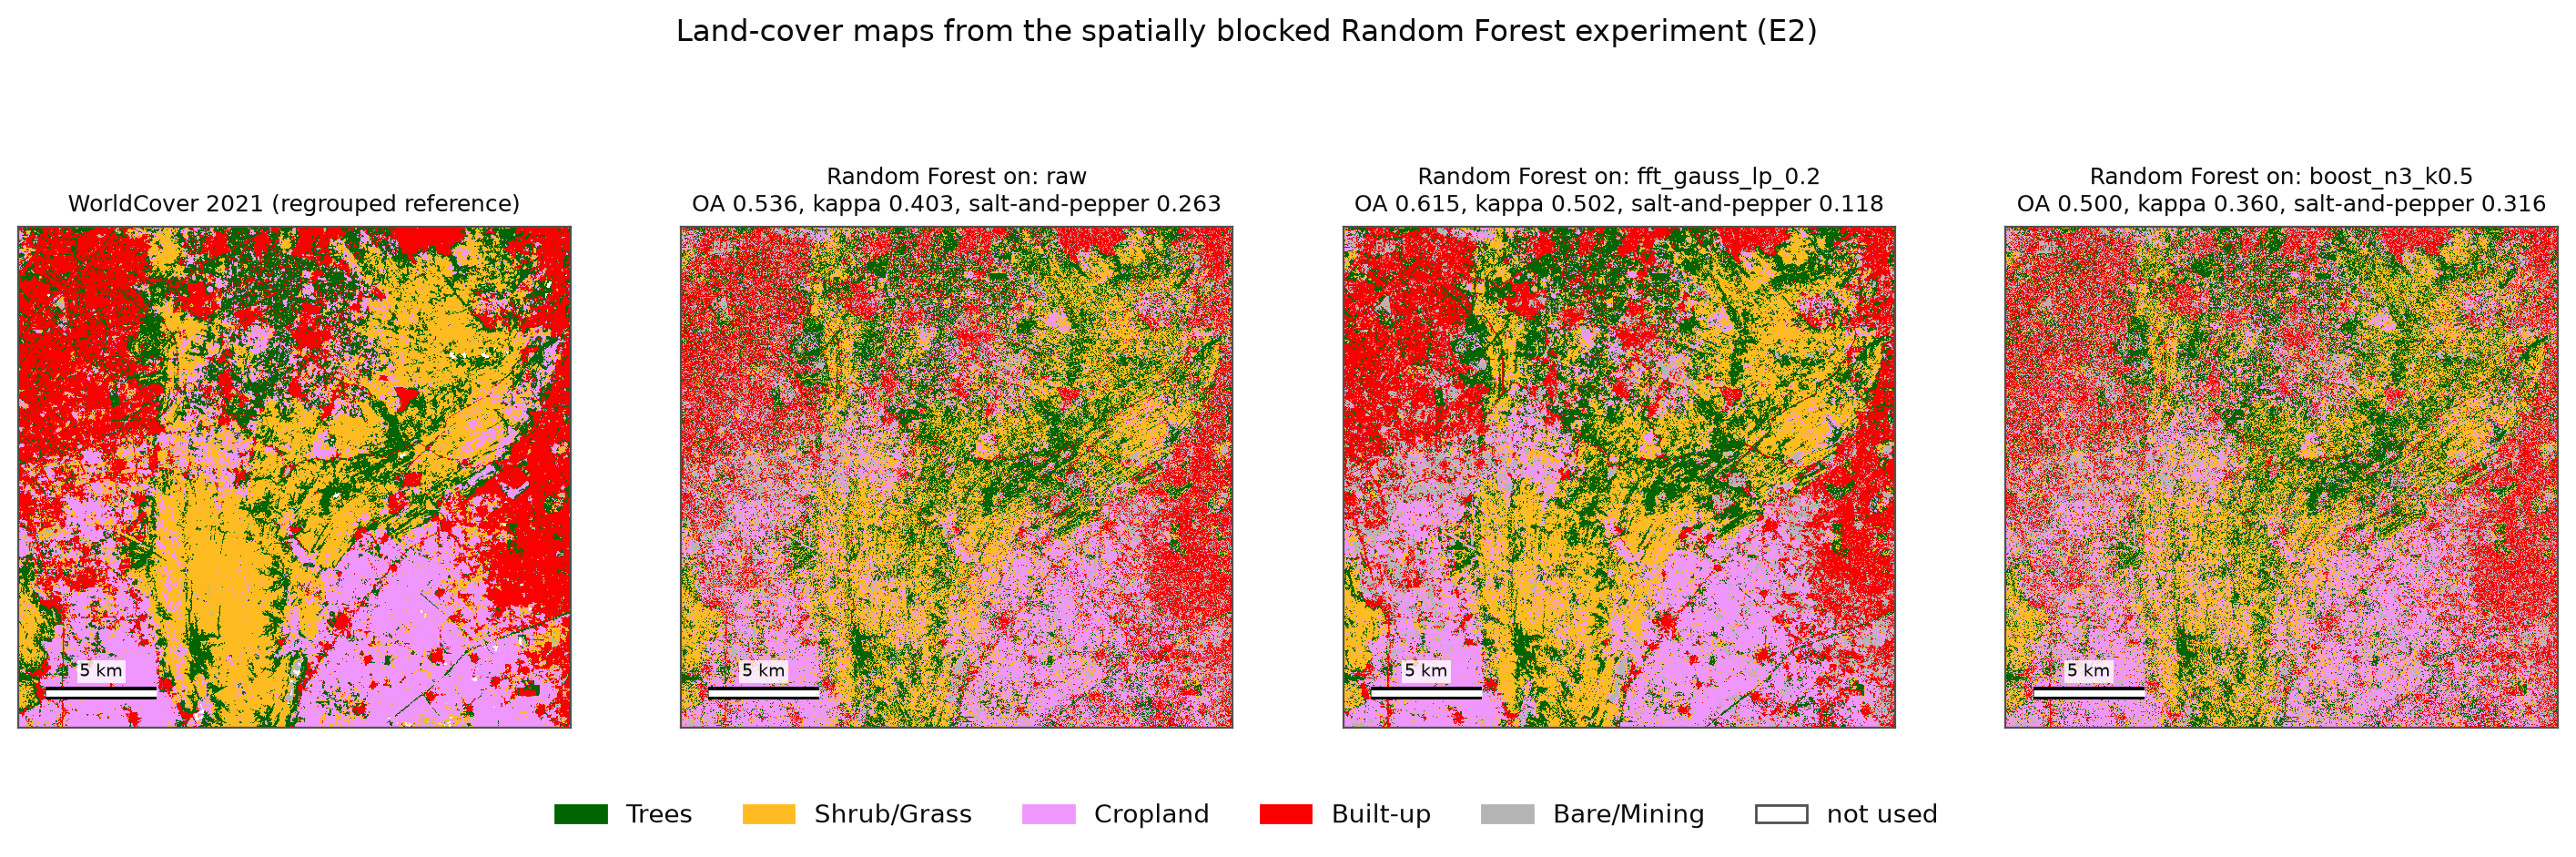
\includegraphics[width=0.84\textwidth]{fig07_classification_maps.png}

\vspace{2pt}
\footnotesize
\begin{tabular}{@{}lcc@{\hspace{7mm}}lcc@{}}
\toprule
\multicolumn{3}{@{}l}{\textbf{E2 classification} ($\kappa$, higher is better)} & \multicolumn{3}{l@{}}{\textbf{E3 edges} (boundary F1, higher is better)} \\
\midrule
No filter & <<e2_raw_kappa>> & speckle <<e2_raw_sp>> & No filter & <<e3_orig_f1>> & \\
Best low-pass & \textbf{<<e2_best_kappa>>} & speckle \textbf{<<e2_best_sp>>} & Best high-boost & \textbf{<<e3_hb_best_f1>>} & \\
Best high-boost & <<e2_hb_best_kappa>> & & Mean $5\times5$ & <<e3_box5_f1>> & \\
\bottomrule
\end{tabular}

\source{Cost: light filters change the spectral angle by <<e4_hb05_sam>>--<<e4_g1_sam>>$^\circ$; a full band takes <<e5_box3>> s with a $3\times3$ kernel and <<e5_fft_min>>--<<e5_fft_max>> s with any FFT mask.}
\end{frame}
\note{[Robin | 1:20 | 8:55]\\
Here a computer classified every pixel into land-cover classes after each filter. From the left: the WorldCover reference, the map from the raw image, from the best smoothed image, and from the best sharpened image. The smoothed map is much cleaner. Its kappa score, which measures agreement with the reference, rose from <<e2_raw_kappa>> to <<e2_best_kappa>>, and the share of isolated speckle pixels fell from <<e2_raw_sp>> to <<e2_best_sp>>. Sharpened images classified worse, because sharpening makes pixels of the same class look more different from each other. For edges the result is reversed: edges found on the sharpened image matched the mapped boundaries best, <<e3_hb_best_f1>> against <<e3_orig_f1>> with no filter, while smoothing removed edges and lowered the score. Along the ridge, the Sobel and Prewitt edge filters gave a small gain. The last line is about cost. Light filters hardly change the colours of the image, a spectral angle of only <<e4_hb05_sam>> to <<e4_g1_sam>> degrees. A 3 by 3 filter takes <<e5_box3>> seconds on a full band, and a frequency-domain filter <<e5_fft_min>> to <<e5_fft_max>> seconds whatever its setting, so for the small filters that worked best, the ordinary spatial method is faster. Sangeeta will bring it together.}

% ================================================================== Conclusions (Sangeeta)
\speaker{Sangeeta}
\section{Conclusions}

% ------------------------------------------------------------------ content slide 9
\begin{frame}{Decision: choose the filter by the job}
\centering
\scriptsize
\begin{tabular}{lll}
\toprule
Application & Best filter & Evidence (best vs.\ no filter) \\
\midrule
<<decision_table_slides>>
\bottomrule
\end{tabular}

\vspace{2pt}
\begin{columns}[T, totalwidth=0.96\textwidth]
\column{0.48\textwidth}
\begin{block}{\textcolor{lpcol}{Pixel values feed a calculation}}
\scriptsize light \textbf{Gaussian}; \textbf{median $3\times3$} for spikes
\end{block}
\column{0.48\textwidth}
\begin{block}{\textcolor{hpcol}{Edges and structure are the point}}
\scriptsize \textbf{high-boost} $k=0.5$--1; \textbf{Sobel/Prewitt} layer
\end{block}
\end{columns}
\vspace{2pt}
{\tiny\color{gray} Avoid the ideal mask (ringing) and heavy smoothing. Limits: one scene, one area; WorldCover is a model output; gains of about 0.01 are not a ranking.\par}
\end{frame}
\note{[Sangeeta | 1:00 | 9:55]\\
This table is produced by our code from the experiment results, one best filter per application. The pattern is clear. When the pixel values feed a calculation, such as removing noise or classifying land cover, light smoothing wins: a small Gaussian, or the 3 by 3 median for scattered bad pixels. When the job is about where things change, such as boundaries, ridge lines or looking at the image, sharpening wins: high-boost at a moderate strength, or an edge layer kept beside the original bands. Some gains are large, like the median on noise and smoothing for classification. Others are small, like urban boundaries and the ridge, and we report them as small. Our limits: one winter scene, one area, and a reference map that is itself a model output. So there is no single most suitable filter; the right one depends on the application.}

% ------------------------------------------------------------------ closing (transition)
\begin{frame}[plain, noframenumbering]
\vfill
\centering
{\usebeamercolor[fg]{structure}\Large\bfseries Thank you. Questions?}\\[8pt]
\footnotesize Live demo: \texttt{python -m rsfilter demo} (offline, 512 $\times$ 512 sample)
\vfill
\end{frame}
\note{[Sangeeta | 0:10 | 10:05]\\
Thank you. We are happy to take questions, and we can run the offline demo if you would like to see it.}

% ------------------------------------------------------------------ references (backup)
\section*{References}
\begin{frame}[allowframebreaks, noframenumbering]{References}
\nocite{*}
\tiny
\bibliographystyle{plainnat}
\bibliography{references}
\end{frame}

\end{document}
